\documentclass[10pt]{article}

\setlength{\oddsidemargin}{0.in}
\setlength{\textwidth}{6.5in}
\setlength{\topmargin}{0.in}
\setlength{\textheight}{8.5in}

%usepackage{hyperref}

\usepackage{graphicx}
\usepackage{url}
%\usepackage{chicago}
\usepackage{amsmath}
\usepackage{moreverb}
\usepackage{draftcopy}
\usepackage{multicol}
\usepackage{boxedminipage}
\usepackage{titlesec}
\usepackage{enumitem}
\usepackage{listings}
\usepackage{textcomp}


\RequirePackage{fancyhdr}
\RequirePackage[colorlinks]{hyperref}


\RequirePackage{fancyvrb}
\DefineVerbatimEnvironment{code}{verbatim}{fontsize=\small}

\RequirePackage{color}
%%% Find colors: http://en.wikipedia.org/wiki/List_of_colors
\definecolor{seagreen}{rgb}{0.18, 0.55, 0.34}
\definecolor{orangy}{cmyk}{0.0, 0.58, 0.100, 0.10}
\definecolor{saffron}{rgb}{0.96, 0.77, 0.19}
\definecolor{carmine}{rgb}{0.59, 0.0, 0.09}
\definecolor{chocolate}{rgb}{0.48, 0.25, 0.0}
\definecolor{darkraspberry}{rgb}{0.53, 0.15, 0.34}
\definecolor{electricindigo}{rgb}{0.44, 0.0, 1.00}
\definecolor{oldmauve}{rgb}{0.40, 0.19, 0.28}
\definecolor{blue-violet}{rgb}{0.54, 0.17, 0.89}
\definecolor{blue(pigment)}{rgb}{0.2, 0.2, 0.6}


\def\bookauthor{Dave Doolin}
\def\booklongtitle{The Final Frontier}
\def\wwkeywords{final-frontier}
\def\wwsubject{solar system exploration}
\def\wwslug{final-frontier}

\hypersetup{%
 pdfauthor={\bookauthor},
 pdftitle={\booklongtitle},
 pdfkeywords={\wwkeywords},
 pdfsubject={\wwsubject},
 urlcolor=cyan,
 pdfdisplaydoctitle=true,
 pdfcreator={Website In A Weekend},
 pdfproducer={\LaTeX},
 baseurl={http://mtngrown.github.io/\wwslug},
 breaklinks=false,
}

%%% Document-specific macros
\def\tff{{\em The Final Frontier}}

\title{The Final Frontier: Man's Expansion Into the Solar System\\
\vspace{2 mm} {\Large Commentary and clarifications on Rules of Play}}
%\subtitle{Commentary and clarifications on Rules of Play}
\date{\today}
\author{mtngrown}


\begin{document}

\maketitle
\tableofcontents


\begin{multicols}{2}

\section{Introduction}

Teaching oneself any sort of intellectually challenging material can be
difficult. When everything is stuck in one's head, it's hard to remember
what's what. Writing out clarifications and commenting on game play helps
me remember rules, and integrate the rules into game play.

The structure of the commentary follows the structure of the games rules,
but does not copy the rules word for word. In some places, selected rules may
be quoted to provide context for clarification.

Some sections may not have any commentary, and exist to preserve the order
of the rules.

Some disclaimers: nothing in this commentary should be considered canonical
with respect to the rules of play, these are strictly my interpretations based
mostly on solo games. The game itself is copyright Kerry Anderson. This
commentary is copyrighted under an attribution license. Copy it, but don't
claim it as your own work.


\section{Game Components}

Most wargame rules have an counter images illustrating the meaning of values,
abbreviations and symbols on the counters. \tff\ does not! In a
spirit of contribution, here is an illustration of a counter, with the associated
explanation.

\begin{center}
  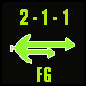
\includegraphics[width=100pt]{../../source/images/final-frontier-frigate.pdf}
\end{center}

\begin{itemize}
  \item ``FG'' stands for Frigate.
  \item The top row of numbers are ordered by Beam - Missile - Damage value.
  \item Any bottom number would be a surface combat value.
\end{itemize}

\section{Preparation For Play}


\tff\ comes in a fairly small box, which is well-packed with counters,
game aids and map. That said, these little components unpack to certain
amount of table space. The main game with the planetary display, the
Economics chart, the Random Events table and the Production Costs
table will fit very nicely under a 24" by 24" plexi. If your table is
big enough to hold a 24" by 36" plexi (wargamer's standard), you're good
to go.

\begin{center}
  PLACEHOLDER FOR GAME IN PROGRESS.
\end{center}

As you can see, all the game parts fit together nicely under a piece of plexi.

\section{Sequence Of Play}

Before each turn, advance the planets according to the Turn Track. Then for
each faction, conduct the turn in the following phase order:

\begin{enumerate}
  \item Economics phase: compute income, adjust Gross National Product (GNP) and
    determine Build Points from cross-referencing National Interest to GNP.
  \item Space movement phase
  \item Space combat phase
  \item Space-surface interaction
  \item Surface combat
  \item Repeat for each player
\end{enumerate}

The early turns of the game will be centered around Economics and Space movement.
It's probably not smart to build warships too early, as they just consume resources
without producing income.


\section{Planets}
\section{Economics}


The economics phase is pretty simple. The complexity is induced
by the unclear explanation of the single entry bookkeeping ledger
supplied with the game.

Some hints:

* The ``income'' column is the total from all resources coming in from mines
and colonies. This number is entered first.

* The GNP is updated by adding the income to the Base GNP.

* The ``Total'' column tracks the Build Points, which are best recorded
as an explicit sum of the current Build Point allotment cross-referenced
from GNP and NI, and the remainder BPs from the previous turn. For example,
suppose 1 BP left over and 3 are allotted. Record this in the ``Total'' column
as ``3 + 1'' instead of ``4.''.

\section{Political Events}
\subsection{National Interest Level}
\subsection{Colonization}

\section{Space Movement}

\section{Space Combat}

\section{Space-Surface Interaction}

\section{Surface Combat}

\section{Earth}

\section{Random Events}

\section{Victory Conditions}

\section{Designer's Notes}

\section{Game Credits}


\section{FAQs and more}

\subsection{National Interest Level}

\begin{itemize}
  \item NI never decreases.
  \item NI increases one step when the the population level of the the largest
    population counter (mine or colony) increases one step. See Section 7.2.
  \item Emplacing the first mine does not increase the NI.
  \item (House rule) The NI is increased when the colony is emplaced, not when
    it is built. This would be a good question for the forums.
\end{itemize}
\section{Summary}

\end{multicols}

\appendix

\section{House rules}

One of the greatest things about having electronic copies of game rules
is it allows players who don't own the game to read up on the rules in
advance of playing an opponent who has the game. While there aren't any
electronic copies of \tff, these notes and the following house rules can
help bridge that gap.

At the moment, these are some notes on what may be some good house rules.

\begin{itemize}
  \item Update Base GNP after every 6th turn by adding the average GNP
    for each turn over the course of the previous six. This will speed up
    the game, but it might also induce a "runaway leader" risk.
\end{itemize}

\section{Player aids}

\subsection{A better ledger}

The ledger which ships with the game is confusing, as it tracks GNP and
Build Points in the same rows, without clearly explaning how the columns
should be used. Compounding this is the problem with any single entry system,
how best to carry balances forward.

\subsection{Status record}

\tff\ lends itself to solo play, and even better, lends itself
to play over time. The game system is simple enough to keep a record of
which pieces are in play, and what their status is, with a handy status
record.

The status record also records the position on the planets.

\subsection{Counter re-creation}

The counters as shipped are 7/16" square. I'm ``re-creating'' a few of the
counters for game play aid using Inkscape, and saving in SVG format.

{\tt DISPLAY= inkscape final-frontier-frigate.svg --export-pdf=final-frontier-frigate.pdf}

Some notes on the ship counters:

\begin{itemize}
  \item The font, evidently, is Compacta, but not bold. That said, Compacta Bold
    is a pretty close fit.
  \item For a nominal 5/8" counter, set the numbers at the top to 12 pt, the letters
    denoting ship type to 11 pt.
  \item With Inkscape, the font stroke should be set to zero, using the fill color to
    draw out the glyphs.
  \item On the ship outlines, set the stroke color to white, which provides a subtle pop
    to the silhouette.
  \item The stroke width on the ships is ???
\end{itemize}

The colors can be approximated using RGB values:

\begin{itemize}
  \item Chartreuse: \#c6ee2b, hsl(72,85,55), rgb(198,238,43)
  \item Magenta: \#f44aad, hsl(325,88,62), rgb(244,74,173)
  \item Cyan: \#a1e2f4, hsl(193,79,79), rgb(161,226,244)
  \item Yellow: \#ffff19, hsl(60,100,54), rgb(255,255,25)
\end{itemize}

\end{document}
